\chapter{Background}\label{chap:background}

This chapter aims to summarize the relevant theory and mathematics of
convolutional networks,
static and dynamic texture synthesis, image style transfer, and representations of dynamics so as to provide sufficient
background information for the following chapters. Research
related to this thesis is covered simultaneously.

\section{Convolutional networks}

A convolutional network (ConvNet) is a feed-forward computational graph of processing nodes, commonly used in analyzing visual imagery. It is a class of artificial neural networks (ANNs), which are computational systems inspired by biological neural networks. ConvNets perform tasks (\eg, object classification) by processing an input, $\mathbf{X} \in \mathbb{R}^{H_x \times W_x \times C_x}$, in a feed-forward manner via a series of linear and non-linear transformations and producing an output, $\mathbf{Y} \in \mathbb{R}^{H_y \times W_y \times C_y}$, relevant to the task (such as the class of an object). Here, $H_\ast \times W_\ast$ represents the spatial dimensions and $C_\ast$ represents the number of channels (\ie, the ``depth'' of the input). For example, a $3$-channel colour image input with $256 \times 256$ spatial locations is represented as $\mathbf{X} \in \mathbb{R}^{256 \times 256 \times 3}$, where each spatial location contains three pixel intensities, corresponding to the amount of intensity of the colours Red, Green, and Blue (RGB), respectively. Each non-linear transformation acts as a point of demarcation in the network known as a \emph{layer}. ConvNets typically consist of multiple layers, each containing a collection of nodes sometimes called \emph{neurons}. At each spatial-channel location of the input to a layer, a neuron computes local non-linear transformations, \eg, $\sigma(\mathbf{x}) = \max{(0, \phi(\mathbf{x}))}$ (known as the \emph{rectified linear unit} or ReLU \cite{nair2010rectified}). At a single location of the input, $\mathbf{x} \equiv (x, y, z)$, the non-linear transformation performed by this neuron produces an output called an \emph{activation} or \emph{feature}, $\sigma(\mathbf{x}) \in \mathbb{R}$. The set of activations produced by a neuron at every location of the input is known as an \emph{activation map} or \emph{feature map}, $\sigma \in \mathbb{R}^{H_\sigma \times W_\sigma \times C_\sigma}$. At the $l$-th layer of the network and for each location $\mathbf{x}$ of the input map, the input to each neuron is the weighted linear combination of activations from neighbouring neurons at the previous layer, $l-1$:
\begin{equation}
	\begin{aligned}
		\phi^l(\mathbf{x}) &= \left(\mathbf{w}^l * \sigma^{l-1}(\mathbf{x})\right) + b^l\\
		&= \left(\sum_{(i, j, k) \in \Omega} \mathbf{w}^l(i, j, k) \sigma^{l-1}(x - i, y - j, z - k)\right) + b^l\ ,
	\end{aligned}
\end{equation}
where $\mathbf{w}^l$ are the \emph{weights} (or \emph{filter}) of the neuron applied to the input $\sigma^{l-1}(\mathbf{x})$, $\Omega$ is a spatial-channel neighbourhood centered about $\mathbf{x}$, $b^l$ is an offset term known as the \emph{bias}, and $\ast$ represents the \emph{convolution} (or \emph{filtering}) operator. Colloquially, the term ``convolution'' is often used to describe the combined process of convolving over an input and subsequently computing its activation. Convolution is typically done in a sliding window fashion across the entire input. At the base of the ConvNet, inputs are typically images while inputs at intermediate layers are activation maps (\eg, $\sigma \in \mathbb{R}^{H_\sigma \times W_\sigma \times C_\sigma}$). 

ConvNets ``learn'' to perform tasks through an iterative process called \emph{training}, which involves optimizing their weights based on an objective over training data (\eg, input images with corresponding expected outputs). At each iteration, an input is fed through the network to produce an output which is subsequently evaluated against the expected, \ie, ``true'', output for the given input. This evaluation is known as the \emph{loss function} and represents the network's performance on the task. Implicitly, it also represents the objective the network must achieve, \eg, minimizing classification error. Starting from the loss, the network adjusts its weights and biases at each layer via the gradient of the loss with respect to the weights and biases at that layer. After a suitable amount of training iterations, this \emph{gradient descent} process is terminated.

\section{Parametric texture synthesis}

Texture synthesis is the process of algorithmically constructing a texture that
matches or extends a given source texture by taking advantage of its structural 
content. There are two general approaches that have dominated the texture
synthesis literature: non-parametric sampling approaches that
synthesize a texture by sampling pixels of a given source texture
\cite{efros1999,kwatra2003graphcut,schodl2000,wei2000}, and 
statistical parametric models that aim to synthesize a texture by sampling
from a parameterized model of the source texture.
As the proposed approach is an instance of a parametric model, this thesis 
will focus on these parametric approaches.

The statistical characterization of visual textures was introduced
in the seminal work of Julesz \cite{julesz1962}.
He conjectured that particular statistics of pixel intensities
were sufficient to partition textures into metameric (\ie,
perceptually indistinguishable) classes. 
Later work leveraged this notion for static texture synthesis
\cite{heeger1995pyramid,portilla2000parametric}.
In particular, inspired by models of the early stages of visual 
processing, statistics of (handcrafted) multi-scale oriented filter 
responses were used to optimize an initial noise pattern 
to match the filter response statistics of an input texture.

More recently, Gatys \etal \cite{gatys2015} demonstrated
impressive results by replacing the handcrafted linear filter bank with the learned filters from the VGG-19
\cite{simonyan2014very} ConvNet pre-trained on the ImageNet \cite{russakovsky2015} dataset for the task of object
recognition. This ConvNet, in effect, served as a proxy for the ventral visual
processing stream. 
Textures were modelled in terms of the normalized correlations between activation maps within several layers of the network.

\subsection{Texture synthesis using a convolutional network}
\label{sec:texture_synthesis_using_a_convnet}

Since the two-stream approach to dynamic texture synthesis proposed in this thesis is an extension of the Gatys \etal \cite{gatys2015} texture 
synthesis model, it is useful to describe their approach here. Given a target texture as input,
let $\mathbf{A}^{l} \in \mathbb{R}^{N_l\times M_l}$
be its row-vectorized activation maps at the $l$-th layer of a ConvNet, where $N_l$ and $M_l$ denote the number of
activation maps and the number of spatial locations,
respectively (in the case of Gatys \etal \cite{gatys2015}, they used the VGG-19 ConvNet, and they normalized the network by scaling its weights such that the mean activation of each convolutional filter over images and positions is equal to one).
The normalized correlations between activation maps
within a layer are encapsulated by a Gram matrix,
$\mathbf{G}^l \in \mathbb{R}^{N_l \times N_l}$, whose entries are given by:
\begin{equation}
	G_{ij}^l = \frac{1}{N_l M_l} \sum_{k=1}^{M_l} A_{ik}^l A_{jk}^l\ ,
\end{equation}
where $A_{ik}^l$ denotes the activation of feature $i$ at
location $k$ in layer $l$ on the target texture. Note that the Gram matrix assumes spatial invariance of the activation statistics.
Given a synthesized texture as input, similarly, let its row-vectorized activation maps
be $\hat{\mathbf{A}}^{l} \in \mathbb{R}^{N_l\times M_l}$ and its normalized
activation map correlations be the Gram matrix, $\hat{\mathbf{G}}^l \in \mathbb{R}^{N_l \times N_l}$, whose entries are given by:
\begin{equation}
	\hat{G}_{ij}^l = \frac{1}{N_l M_l} \sum_{k=1}^{M_l} \hat{A}_{ik}^l \hat{A}_{jk}^l\ .
\end{equation}
The final objective is defined as the average of the mean squared error between
the Gram matrices of the target texture and that of the synthesized texture:
\begin{equation}
   \mathcal{L} = \frac{1}{L} \sum_{l} \Vert \mathbf{G}^l - \hat{\mathbf{G}}^l \Vert^2_F\ ,
   \label{eq:tex_loss}
\end{equation}
where $L$ is the number of ConvNet layers used when computing Gram matrices
and $\Vert \cdot \Vert_F$ is the Frobenius norm. In the case of Gatys \etal \cite{gatys2015}, Gram matrices were computed on
layers \emph{conv1\_1}, \emph{pool1}, \emph{pool2}, \emph{pool3}, and \emph{pool4}.

Before synthesizing a texture, an initial forward pass through the ConvNet is
performed with the target texture as input. The target texture's Gram matrices
across various layers in the network are computed and stored to be used in the final objective for
the synthesis process (Eq.\ \ref{eq:tex_loss}). Then the synthesized texture is initialized with Independent and Identically Distributed (IID)
Gaussian noise. The final
objective (Eq.\ \ref{eq:tex_loss}) is minimized with respect to the synthesized texture. With each
iteration of the optimization process, the synthesized texture is updated to appear increasingly
perceptually similar to the target texture. An overview of this process is presented in Fig.\ \ref{fig:vgg_texture_synthesis}.
\clearpage
\begin{figure}[t]
\begin{center}
	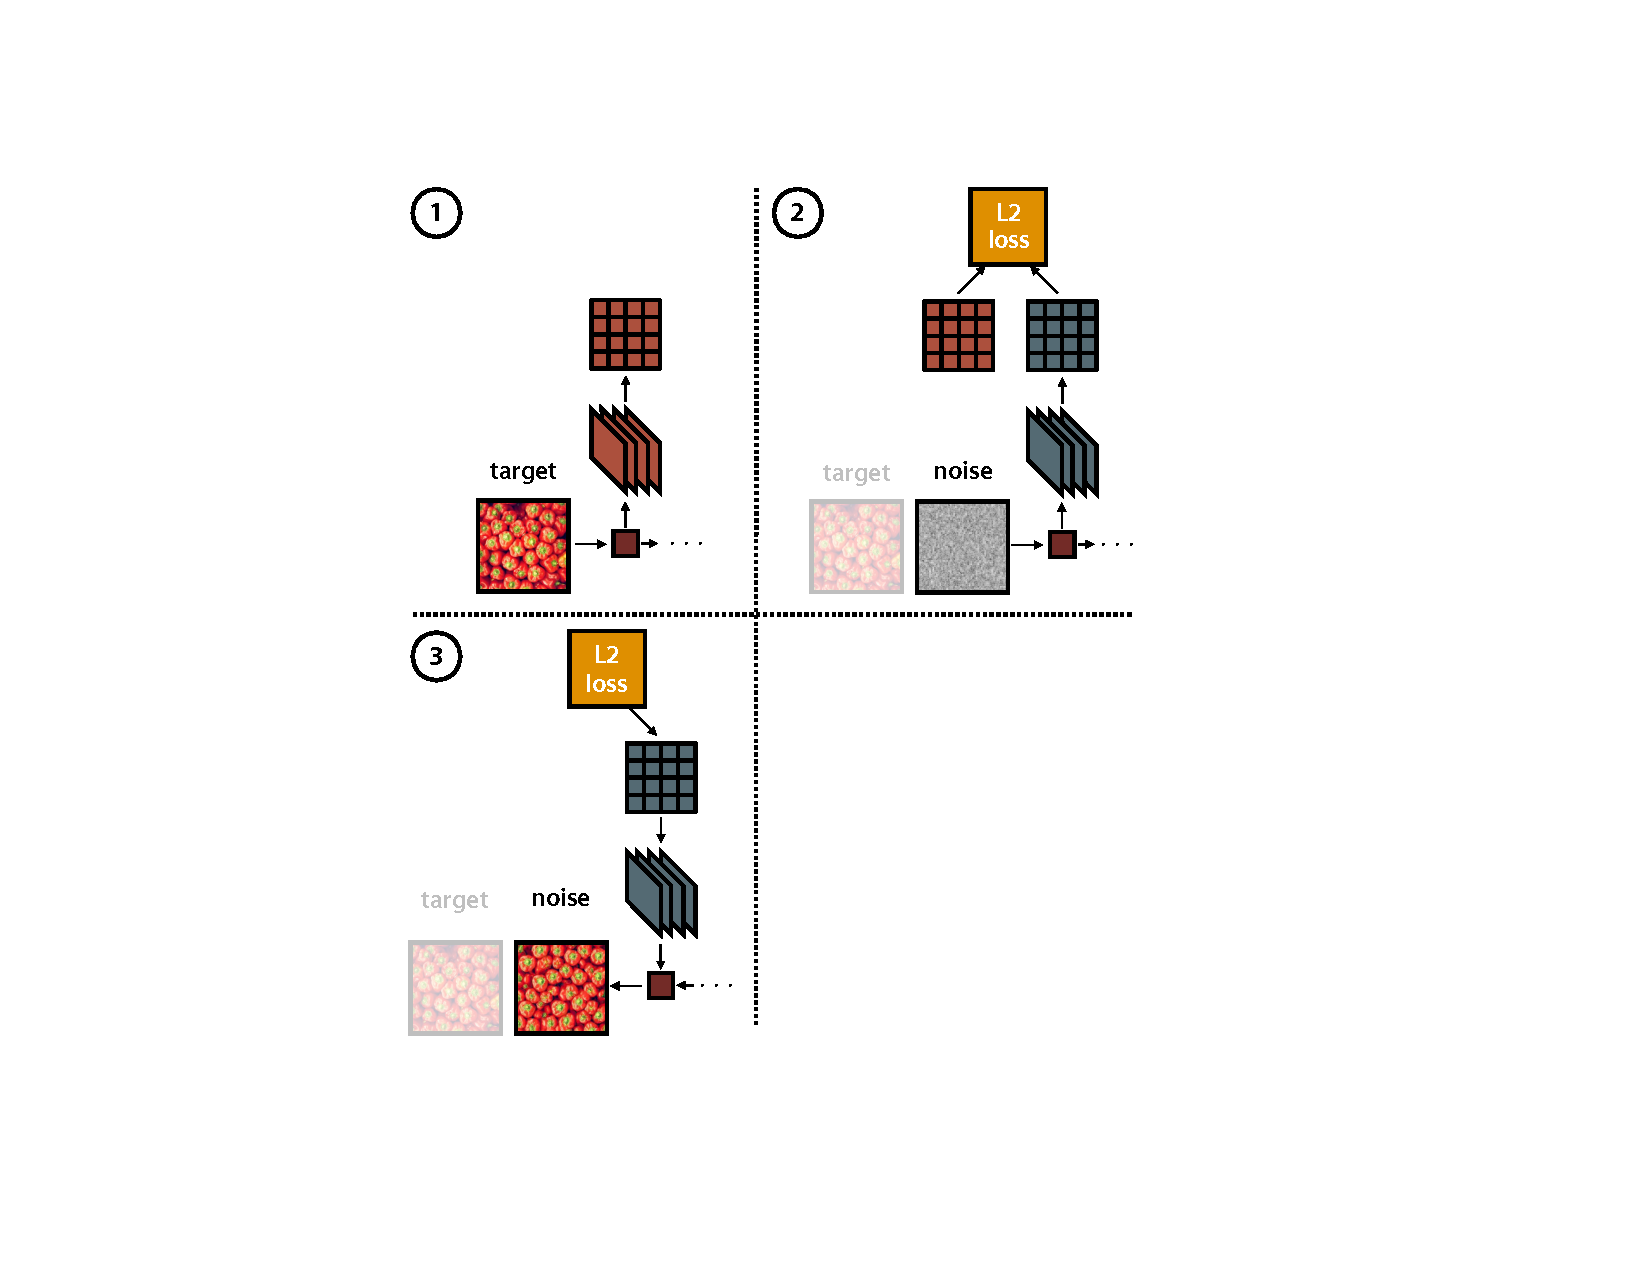
\epsfig{file=vgg_texture_synthesis.pdf, width = \textwidth}\\
	\caption[Static texture synthesis with a convolutional network]{Gatys \etal's \cite{gatys2015} approach to static texture synthesis with the VGG-19 \cite{simonyan2014very} convolutional network. Only the first layer of VGG-19 is shown. (1) An initial forward pass is
performed with the target texture. Its Gram matrices
across various layers are computed and saved. (2) The total L2 loss between the synthesized texture's Gram matrices and the target's is computed. (3) The loss is optimized with respect to the synthesized texture (with the weights of VGG-19 fixed), updating it to appear perceptually similar to the target.}
	\vspace{-0.65cm}
	\label{fig:vgg_texture_synthesis}
\end{center}
\end{figure}
\clearpage

\subsection{The Gram matrix as a texture metric}

Before explaining the Gram matrix as a suitable texture metric, it is necessary to first understand the mathematics behind it. The Gram matrix, $\mathbf{G} \in \mathbb{R}^{n \times n}$, of a set of $m$-dimensional vectors, $v_1, \dots , v_n \in \mathbb{R}^m$, is the symmetric matrix of inner products, whose entries are given by $G_{ij} = \langle v_i, v_j \rangle$. Essentially, the Gram matrix is a covariance matrix describing which of its input vectors are correlated with each other. In the case of Gatys \etal's \cite{gatys2015} texture synthesis with a ConvNet, the set of vectors used to compute the Gram matrix are row-vectorized activation maps (Fig.\ \ref{fig:gram_matrix}).
\begin{figure}[t]
\begin{center}
	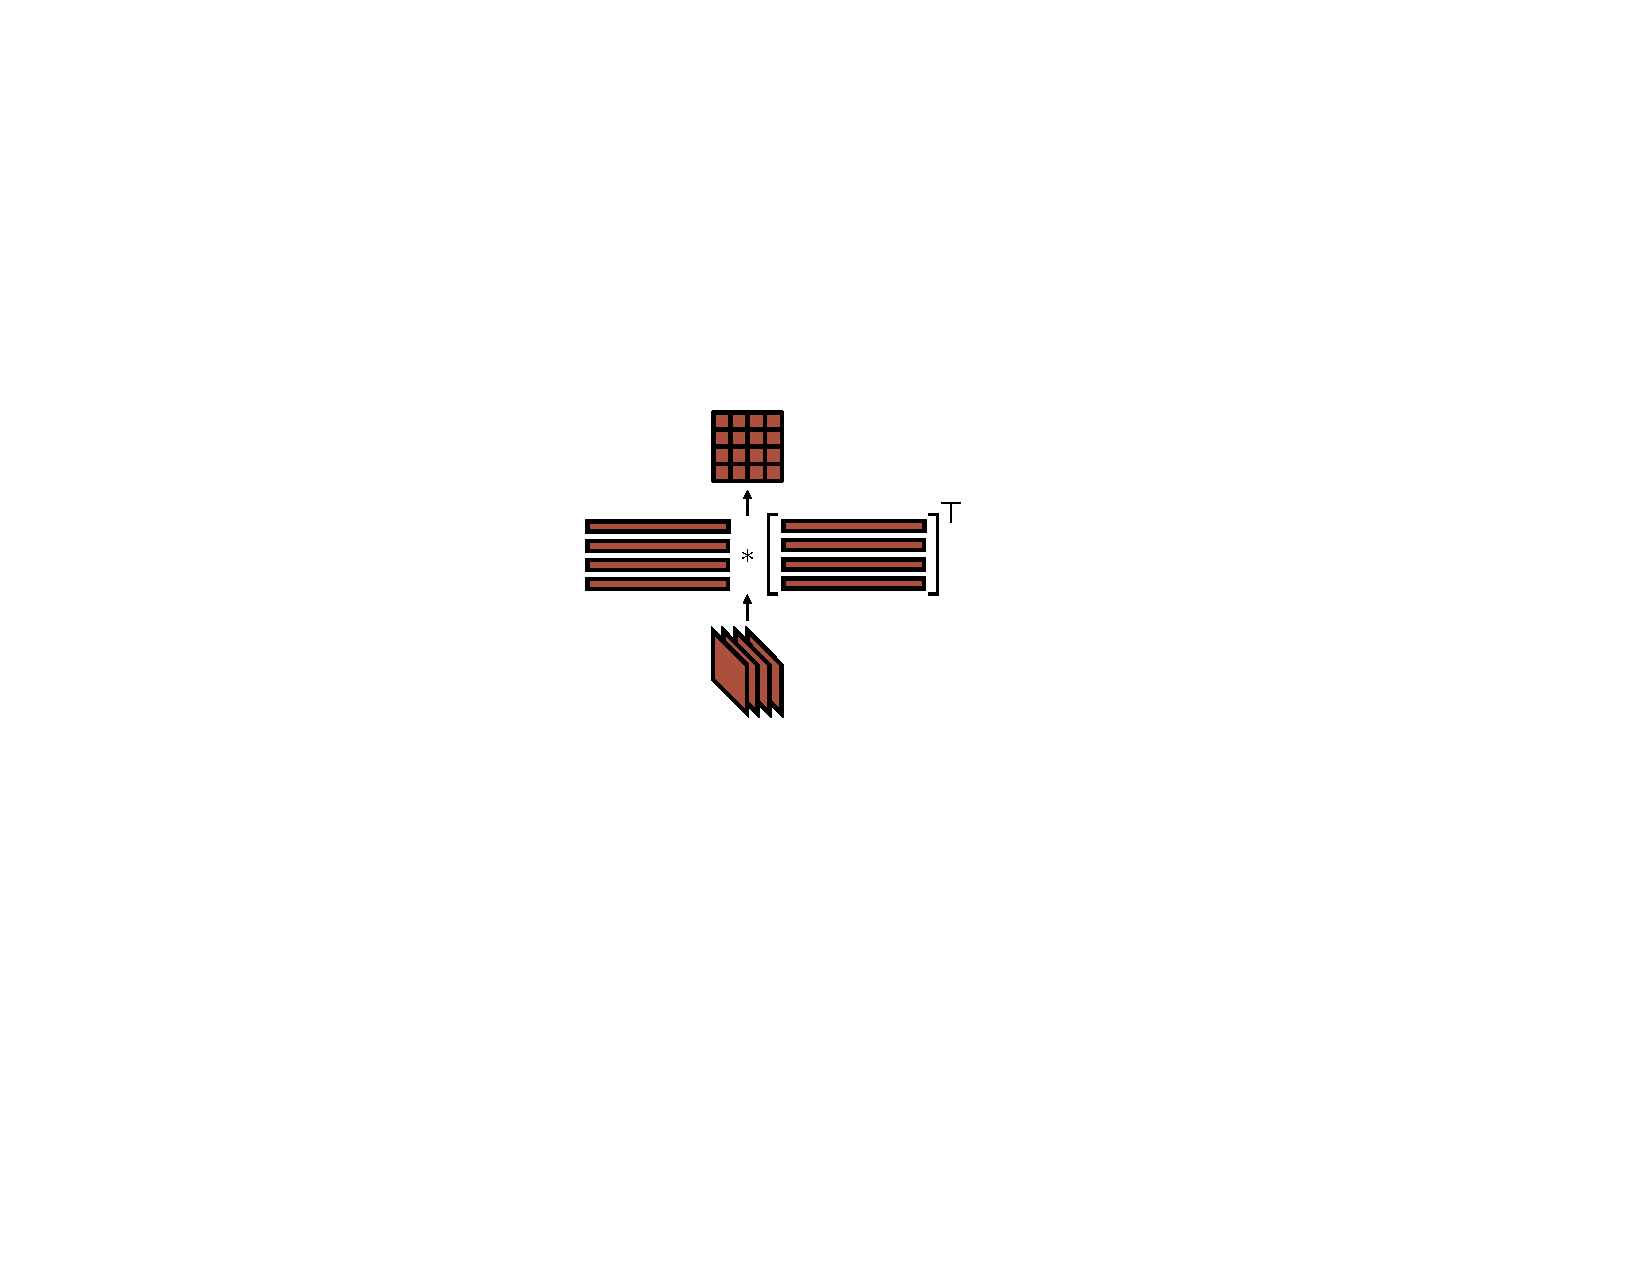
\epsfig{file=gram_matrix.pdf, width = 0.6 \textwidth}\\
	\caption[Computing the Gram matrix from activation maps]{Computing the Gram matrix from the activation maps of a layer. Activation maps are first reshaped to row vectors, then the Gram matrix is realized by computing a matrix multiplication between the row-vectorized activation maps and their transpose.}
	\vspace{-0.65cm}
	\label{fig:gram_matrix}
\end{center}
\end{figure}

In texture synthesis, the Gram matrix measures the amount that co-located features tend to activate together. By computing Gram matrices across several layers, a stationary, multi-scale representation of the input image in terms of its texture information is achieved.

\subsection{Image style transfer}

In subsequent work, Gatys \etal's \cite{gatys2016image} texture model was used in image style
transfer, where the style of one image was
combined with the image content of another to produce a new image.
This was achieved by appending an additional term to Eq.\ \ref{eq:tex_loss}
that enforced the synthesized texture to match the semantic content of the given content image. Specifically,
\begin{equation}
   \mathcal{L} = \frac{1}{L_{style}} \sum_{l} \Vert \mathbf{G}^l - \hat{\mathbf{G}}^l \Vert^2_F\ + \frac{1}{L_{content}} \sum_{l} \Vert \mathbf{A}^l - \hat{\mathbf{A}}^l \Vert^2_F\ ,
   \label{eq:styletransfer_loss}
\end{equation}
where $L_{style}$ and $L_{content}$ are the number of VGG-19 layers used when computing Gram matrices and activation maps, respectively. Gram matrices are computed on the same layers as before, and activation maps are computed on layer \emph{conv4\_2}.

To briefly review, the Gram matrix of activation maps conveys a notion of texture, or ``style'', describing which features tend to activate together. Although the style of the style image is preserved, the global arrangement of its features are not. By including the objective of matching the features of the content image, however, the global arrangement of semantic image content from the content image is preserved. This results in a synthesized image that contains the content of the content image and the style of the style image.

\section{Dynamic texture synthesis}

Dynamic textures extend from static textures with an additional temporal dimension. The stationarity of spatial statistics of static textures also applies to the temporal domain of dynamic textures.

Unlike static texture synthesis, dynamic texture synthesis has not been as deeply explored. Somewhat related to dynamic texture synthesis, Ruder \etal \cite{ruder2016} extended the image style transfer model to video by using
optical flow to enforce temporal consistency of the
resulting imagery. Although their model produced a video output, their core approach focused on an analysis of static texture on a per-frame basis. This is not to be confused with dynamic texture synthesis, which requires an analysis of \emph{dynamic} textures across space \emph{and time}.

Variants of linear autoregressive models have been studied
\cite{szummer1996,doretto2003,wang2003,fitzgibbon2001} that jointly model the appearance and
dynamics of spatiotemporal patterns.
More recent work has considered ConvNets as a basis for modelling 
dynamic textures.
Xie \etal \cite{xie2017synthesizing} proposed a spatiotemporal
generative model where each dynamic texture is modelled as a random
field defined by multiscale, spatiotemporal ConvNet filter responses
and dynamic textures are realized by sampling the model.
Unlike the proposed approach, which assumes pre-trained fixed networks,
Xie \etal's \cite{xie2017synthesizing} approach requires their ConvNet weights to be trained using the input texture prior to synthesis. The manner in which they model dynamic textures appears to limit synthesis to a reconstruction, not an extrapolation, of the original sequence, limiting the generalizability (\eg, synthesis of textures beyond the spatiotemporal extent of the input) of their approach.
A recent preprint from Funke \etal \cite{funke2017} described preliminary 
results extending the framework of Gatys \etal \cite{gatys2015} 
to model and  synthesize dynamic textures by computing a Gram 
matrix of filter activations over a small spatiotemporal window.
In contrast, the proposed two-stream filtering architecture is more 
expressive as the dynamics stream is specifically tuned to 
spatiotemporal dynamics.
Moreover, the factorization
in terms of appearance and dynamics enables a novel form of
style transfer, where the dynamics of one pattern are 
transferred to the appearance of another to generate an
entirely new dynamic texture.
This work is the first to demonstrate this form of style transfer.


\section{Representations of dynamics}

Numerous representations of dynamics in temporal imagery have been explored, each with their own limitations and level of abstraction. Figure \ref{fig:dynamics_representations} illustrates an organization of several extant representations of temporal imagery dynamics.
\begin{figure}[t]
\begin{center}
	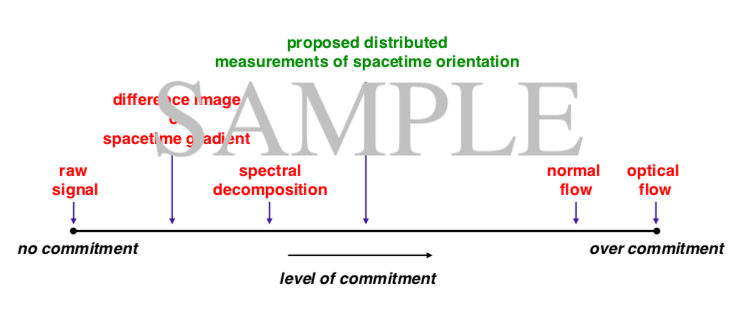
\epsfig{file=dynamics_representations.png, width = \textwidth}\\
	\caption[Dynamics representation spectrum]{Dynamics representation spectrum (adapted from Derpanis \cite{derpanis2010role}). Common abstractions of dynamics of temporal imagery and their respective level of commitment to an underlying model.}
	\vspace{-0.65cm}
	\label{fig:dynamics_representations}
\end{center}
\end{figure}
At one extreme, no commitment to an abstraction is made, the raw pixelwise intensity is used directly. This representation fails to leverage the rich underlying structure in the data. The remaining representations are discussed below.

\subsection{Optical flow}

At the other extreme of Fig.\ \ref{fig:dynamics_representations}, a two-dimensional (2D) vector field is used to represent the dynamics of the input temporal imagery. This vector field is known as \emph{optical flow}. It is used to represent the apparent motion of image pixels between two consecutive frames that is caused by the movement of objects or the camera. Each vector in the 2D vector field is a displacement vector consisting of a horizontal and vertical component, describing the movement of pixels from one frame to the next. Figure \ref{fig:optical_flow} provides a useful visualization of optical flow.
\begin{figure}[t]
\begin{center}
	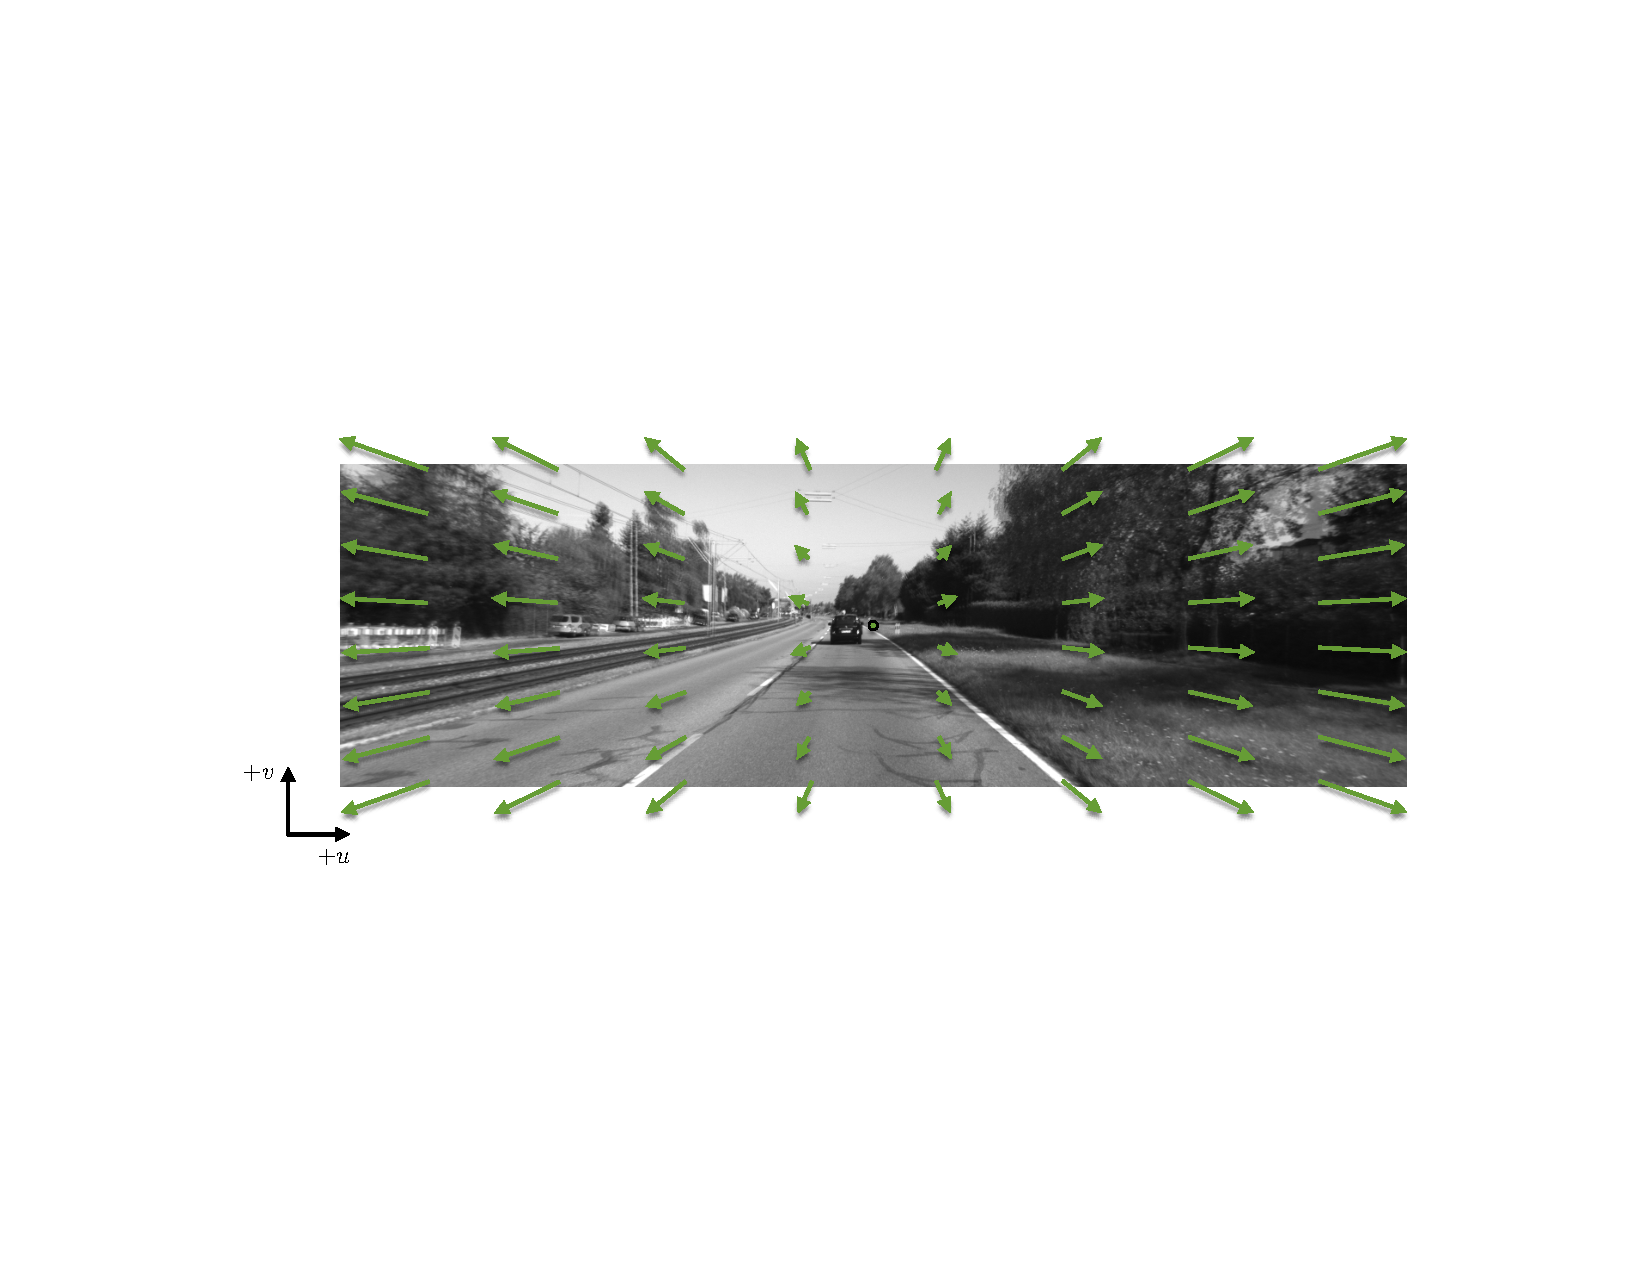
\epsfig{file=optical_flow.pdf, width = \textwidth}\\
	\caption[Optical flow visualization]{Optical flow visualization. Optical flow is a 2D displacement vector field used to represent the apparent motion of image pixels between two consecutive frames, caused by the movement of objects or the camera. Pictured are two, super-imposed, consecutive frames taken from the KITTI dataset \cite{geiger2013vision}. The corresponding optical flow is visualized as an array of green arrows. Note that this is just a sample of the motions that optical flow can characterize.}
	\vspace{-0.65cm}
	\label{fig:optical_flow}
\end{center}
\end{figure}
The recovery of optical flow from temporal imagery has long been studied in computer vision. Traditionally, it has been addressed by handcrafted approaches \eg, \cite{horn1981,lucas1981,revaud2015epicflow}. Recently, ConvNet approaches have been demonstrated as viable alternatives \cite{dosovitskiy2015,ilg2017,ranjan2017,yu2016}.

A limitation of optical flow is its reliance on a single coherent movement for each pixel and its underlying assumption on brightness constancy, which is difficult to justify for the spectrum of dynamics one encounters in the real world. Examples of dynamics that optical flow would fail to capture include flickering, semi-transparent motion, and stochastic dynamics. These are some of the dynamics typically exhibited by dynamic textures. Therefore, optical flow is not an optimal measure for representing the spectrum of dynamics in dynamic textures.

\subsection{Marginalized spacetime oriented energies}
\label{sec:msoe}

At the midpoint between the two extremes lies the representation of dynamics that aims to capture a distribution of measurements of spacetime orientations in the input temporal imagery.
Unlike flow-based analyses which focus on the apparent motion (\ie, translation) present in the data, measurements of spacetime orientations take a geometric and generalized approach in capturing \emph{spacetime structures}: oriented structures in the spatiotemporal domain that manifest themselves as motion or non-motion (\eg, flickering, stochastic dynamics, etc.).

Previous works \cite{adelson1985spatiotemporal,fahle1981,heeger1988,simoncelli1998,watson1983,nishimoto2011,derpanis2012spacetime} have shown that the velocity of image content (\ie, motion) is interpreted as a 3D oriented structure in the $x$-$y$-$t$ spatiotemporal domain. Furthermore, in the frequency domain, they showed that the signal energy of these oriented structures lie on a plane through the origin where the slant of the plane is defined by the velocity of the image content.
For example, in the case where a spacetime structure is defined by the image velocity $(u, v)^\top$, the unit normal of the plane is given by $\hat{\mathbf{n}}=(u, v, 1)^\top / ||(u, v, 1)^\top||$.
Hence, energy models of visual motion, like those presented in these works, are described as ``oriented energy'' or ``motion energy'' models, and they attempt to identify this orientation-plane (and hence the pattern's velocity) via a set of image filtering operations. Specifically, given an input image sequence, these models consist of an alternating sequence of linear and non-linear operations that yield a distributed representation (\ie,  implicitly coded) of pixelwise
optical flow. These models have been motivated and studied in a variety of contexts, including computer vision, visual neuroscience, and visual psychology

Whereas motion indicates a single, dominant orientation in the spatiotemporal and frequency domains, non-motion can indicate an unconstrained, underconstrained, multi-dominant, heterogeneous, or isotropic orientation. For example, an unconstrained orientation corresponds to structure-less imagery (\eg, image of a clear sky) in the spatiotemporal domain and a structure-less energy response in the frequency domain; and a multi-dominant orientation corresponds to multiple, super-imposed spacetime structures in the spatiotemporal domain (\eg, waterfall over a stationary background) and multiple, super-imposed oriented planes in the frequency domain. These, along with the other orientations, are visualized in Fig.\ \ref{fig:spacetime_structures}.
\clearpage
\begin{figure}[t]
\begin{center}
	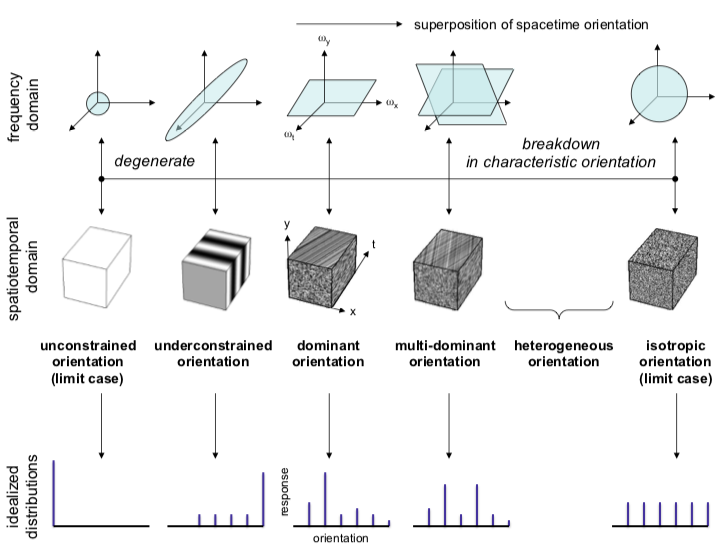
\epsfig{file=spacetime_structures.png, width = \textwidth}\\
	\caption[Spacetime texture spectrum]{Dynamic texture spectrum (adapted from Derpanis \cite{derpanis2012spacetime}). The top and middle rows depict prototypical dynamic textures in the frequency and spatiotemporal domains, respectively. From left-to-right, an increasing amount of spacetime structures are superimposed in a texture. The bottom row depicts a seven bin histogram of the relative spacetime-oriented structure (or lack thereof) present in each dynamic texture. The first histogram bin captures lack of structure. The remaining histogram bins from left-to-right correspond to spacetime orientations selective for static, rightward motion, upward motion, leftward motion, downward motion and flicker structure.}
	\vspace{-0.65cm}
	\label{fig:spacetime_structures}
\end{center}
\end{figure}
\clearpage

This thesis adopts the Marginalized Spacetime Oriented Energy (MSOE) approach of Derpanis and Wildes \cite{derpanis2012spacetime} in representing the observed distribution of dynamics (\ie motion and non-motion) of an input dynamic texture. They conjectured that the constituent spacetime orientations for a spectrum of common
visual patterns (\eg, dynamic textures) can serve as a basis for describing the temporal
variation of an image sequence. They successfully applied their model for the task of dynamic texture recognition; here it is used for the task of dynamic texture synthesis. Significantly, a completely analytically-defined
oriented energy ConvNet model provides the current state-of-the-art
for the related task of dynamic texture recognition \cite{hadji2017}. The proposed two-stream architecture adopts the MSOE model by encoding it as a ConvNet that serves as the representation of observed dynamics of input dynamic textures---the dynamics stream. The same computational steps are used, however, the handcrafted filters of the MSOE model are not used and are learned instead. The construction of the ConvNet is discussed in the next chapter and the MSOE model is reviewed here.

Given input temporal imagery, $\mathbf{I} \in \mathbb{R}^{T \times H \times W}$ (time $\times$ height $\times$ width), a bank of oriented 3D
filters, \eg, Gaussian third derivative filters $G_3 \in \mathbb{R}^{T \times H \times W}$, which are sensitive to a range of
spatiotemporal orientations, are each applied:
\begin{equation}
	E_{\hat{\theta}} = G_{3_{\hat{\theta}}} \ast \mathbf{I}\ ,
\end{equation}
where $\ast$ denotes convolution, and $G_{3_{\hat{\theta}}}$ is a Gaussian third derivative filter oriented in the direction of the 3D unit vector $\hat{\theta}$ which lies along the filter's symmetry axis. Each of these filtering operations results in a spacetime volume of filter responses, $E_{\hat{\theta}}$.
These filter responses are then rectified (squared) and
pooled over local spacetime regions to make the responses robust
to the phase of the input signal, \ie, robust to the
alignment of the filter with the underlying image
structure:
\begin{equation}
	\bar{E}_{\hat{\theta}} = \sum_{(x, y, t) \in \Omega}{{E_{\hat{\theta}}(x, y, t)}^2}\ .
\end{equation}
At this point, each oriented energy measurement includes measurement of spatial orientation. This means that spatial image structures will affect the responses of the bank of oriented filters, making them dependent on spatial appearance. This is unwanted as this interference can occur at an otherwise coherent dynamic region, \eg, a surface with varying spatial appearance exhibiting a single, dominant motion. Thus, a description consisting purely of pattern dynamics is sought.
To remove this difficulty, the spatial orientation component of each filter is discounted via ``marginalization''. Specifically, filter responses consistent with the same temporal orientation (not necessarily the same spatial orientation), $\hat{\theta}_i$, are summed:
\begin{equation}
	E_{\hat{\mathbf{n}}} = \sum_{i = 1}^{N}{E_{\hat{\theta}_i}}\ ,
	\label{eq:oriented_filter_2.8}
\end{equation}
where $\hat{\mathbf{n}}$ denotes the unit normal of the plane in frequency-space that the spacetime structures captured by these filters lie upon (implicitly describing a single temporal orientation), and $N$ denotes the number of these filters.
These responses provide a pixelwise distributed measure
of which spacetime structures (discounting spatial information) are
present in the input.
However, these responses are confounded by local image
contrast that makes 
it difficult to determine
whether a high response is indicative of the presence of
a spacetime structure or simply due to high image
contrast.
To address this ambiguity, an $\textrm{L}_1$
normalization is applied across oriented filter responses which
results in a representation that is robust to local
appearance variations but highly selective to 
spacetime orientation:
\begin{equation}
	\hat{E}_{\hat{\mathbf{n}}_i} = \frac{E_{\hat{\mathbf{n}}_i}}{\sum_{j = 1}^{M}{E_{\hat{\mathbf{n}}_j}} + \epsilon} \ ,
\end{equation}
where $\hat{E}_{\hat{\mathbf{n}}_i}$ denotes an oriented filter response from Eq.\ \ref{eq:oriented_filter_2.8} corresponding to a plane in frequency-space with unit normal $\hat{\mathbf{n}}_i$.